% Latex Beamer template following CERN template guidelines (or trying!)

\documentclass[aspectratio=169]{beamer}
\usepackage{xcolor}
\usepackage{graphicx}
\usepackage{multicol}
\usepackage{tikz}

% Code listings with syntax highlighting
%  Require Pygments
\usepackage{minted}
\usepackage{siunitx}
\usepackage{comment}
\sisetup{output-exponent-marker=\ensuremath{\mathrm{e}}}


\usetheme{CERN}

\newcommand{\interludeTitle}{}
\AtBeginSection[] {
    \frame{
	\frametitle{\interludeTitle}
      \begin{multicols}{2}
        \tableofcontents[
            currentsection,
            sectionstyle=show/shaded,
            ]
	  \end{multicols}
    }
}

\AtBeginSubsection[] {
	  \frame{
		\frametitle{\interludeTitle}
		\begin{multicols}{2}
        \tableofcontents[
            currentsubsection,
            subsectionstyle=show/shaded,
            ]
		\end{multicols}
	  }
}


% Talk date
% Uncomment this to define a presentation date distinct from \today
\def\mydate{11 Oct 2018}

% Preamble
\title[]{Readout System Enhancements for ATLAS ITk Project }
\subtitle{}
\author[Kyle Beyer , Dylan Hatch]{Kyle Beyer, \texorpdfstring{\url{kyle.beyer@cern.ch} \\ Dylan Hatch,  \url{dylan.brown.hatch@cern.ch}}{Kyle Beyer , Dylan Hatch}}

% Body
\begin{document}

    \cernSplashBlue

    % Title
    {
    \setbeamertemplate{footline}{}
    \setbeamertemplate{navigation symbols}{}
    \frame{\titlepage
      \begin{tikzpicture}[remember picture, overlay]
        \node[anchor=south west, %anchor is bottom left corner of the graphic
              xshift=0.5cm, %shifting around
              yshift=0.5cm]
       at (current page.south west) %left bottom corner of the page
        { 
\includegraphics[width=0.3\paperwidth]{images/mlogo.png} };

        \node[anchor=south east, %anchor is bottom left corner of the graphic
              xshift=-0.5cm, %shifting around
              yshift=0.3cm]
       at (current page.south east) %left bottom corner of the page
        {	
\includegraphics[width=0.23\paperwidth]{images/wlogo.png} };
			\end{tikzpicture}
    }
  }

    \setcounter{framenumber}{0}


    % TOC
     \frame{
        \frametitle{Agenda}
        \begin{multicols}{2}
            \tableofcontents
        \end{multicols}
    }

    \section{Background}
    
    \subsection{ATLAS \& the Inner Detector}

    
    % ============================================================== %
    %
    % ATLAS & Inner Detector
    %
    % ============================================================== %

    \frame{
      \frametitle{ATLAS \& the Inner Detector}
    
    }
    
    \subsection{HL-LHC \& ITk}
    

    % ============================================================== %
    %
    % HL-LHC & ITK Frame
    %
    % ============================================================== %
    
    \frame{
      \frametitle{High Luminosity LHC \& ITk Upgrades}
      %

        \begin{columns}[T,onlytextwidth]
        \begin{column}{.54\textwidth}

        \begin{block}{ $x10$ increase in instantaneous luminosity! }
            \begin{itemize}
              \item $L = $\num{1e73} fb$^{-1}$ s$^{-1} \rightarrow 
                     L = $ \num{1e74} fb$^{-1}$ s$^{-1} $ \\
            \end{itemize}
          \end{block}

        \end{column}
        \begin{column}{.4\textwidth}
				\vspace{-1.2cm}
					\begin{figure}
						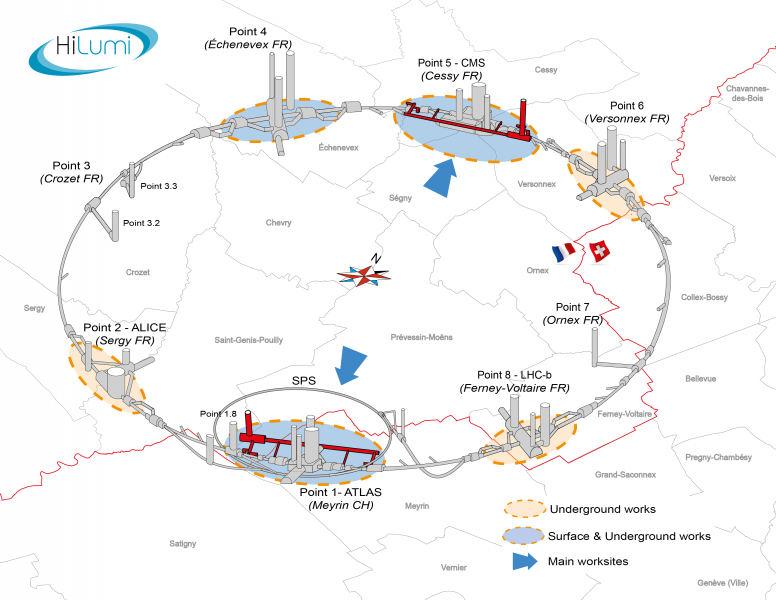
\includegraphics
						[width=\textwidth, height=.4\textheight]
						{p1-figs/hl-upgrade.png}
				 	\end{figure}

        \end{column}
        \end{columns}

        \vspace{-0.1cm}

        \begin{minipage}{\textwidth}
          \begin{columns}[T,onlytextwidth]
          \begin{column}{.5\textwidth}
            \begin{figure}
              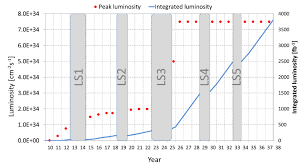
\includegraphics
              [height=.47\textheight]
              {p1-figs/hl.png}
            \end{figure}
          \end{column}
          \begin{column}{.6\textwidth}
            \vspace{0.5cm}
            \begin{figure}
              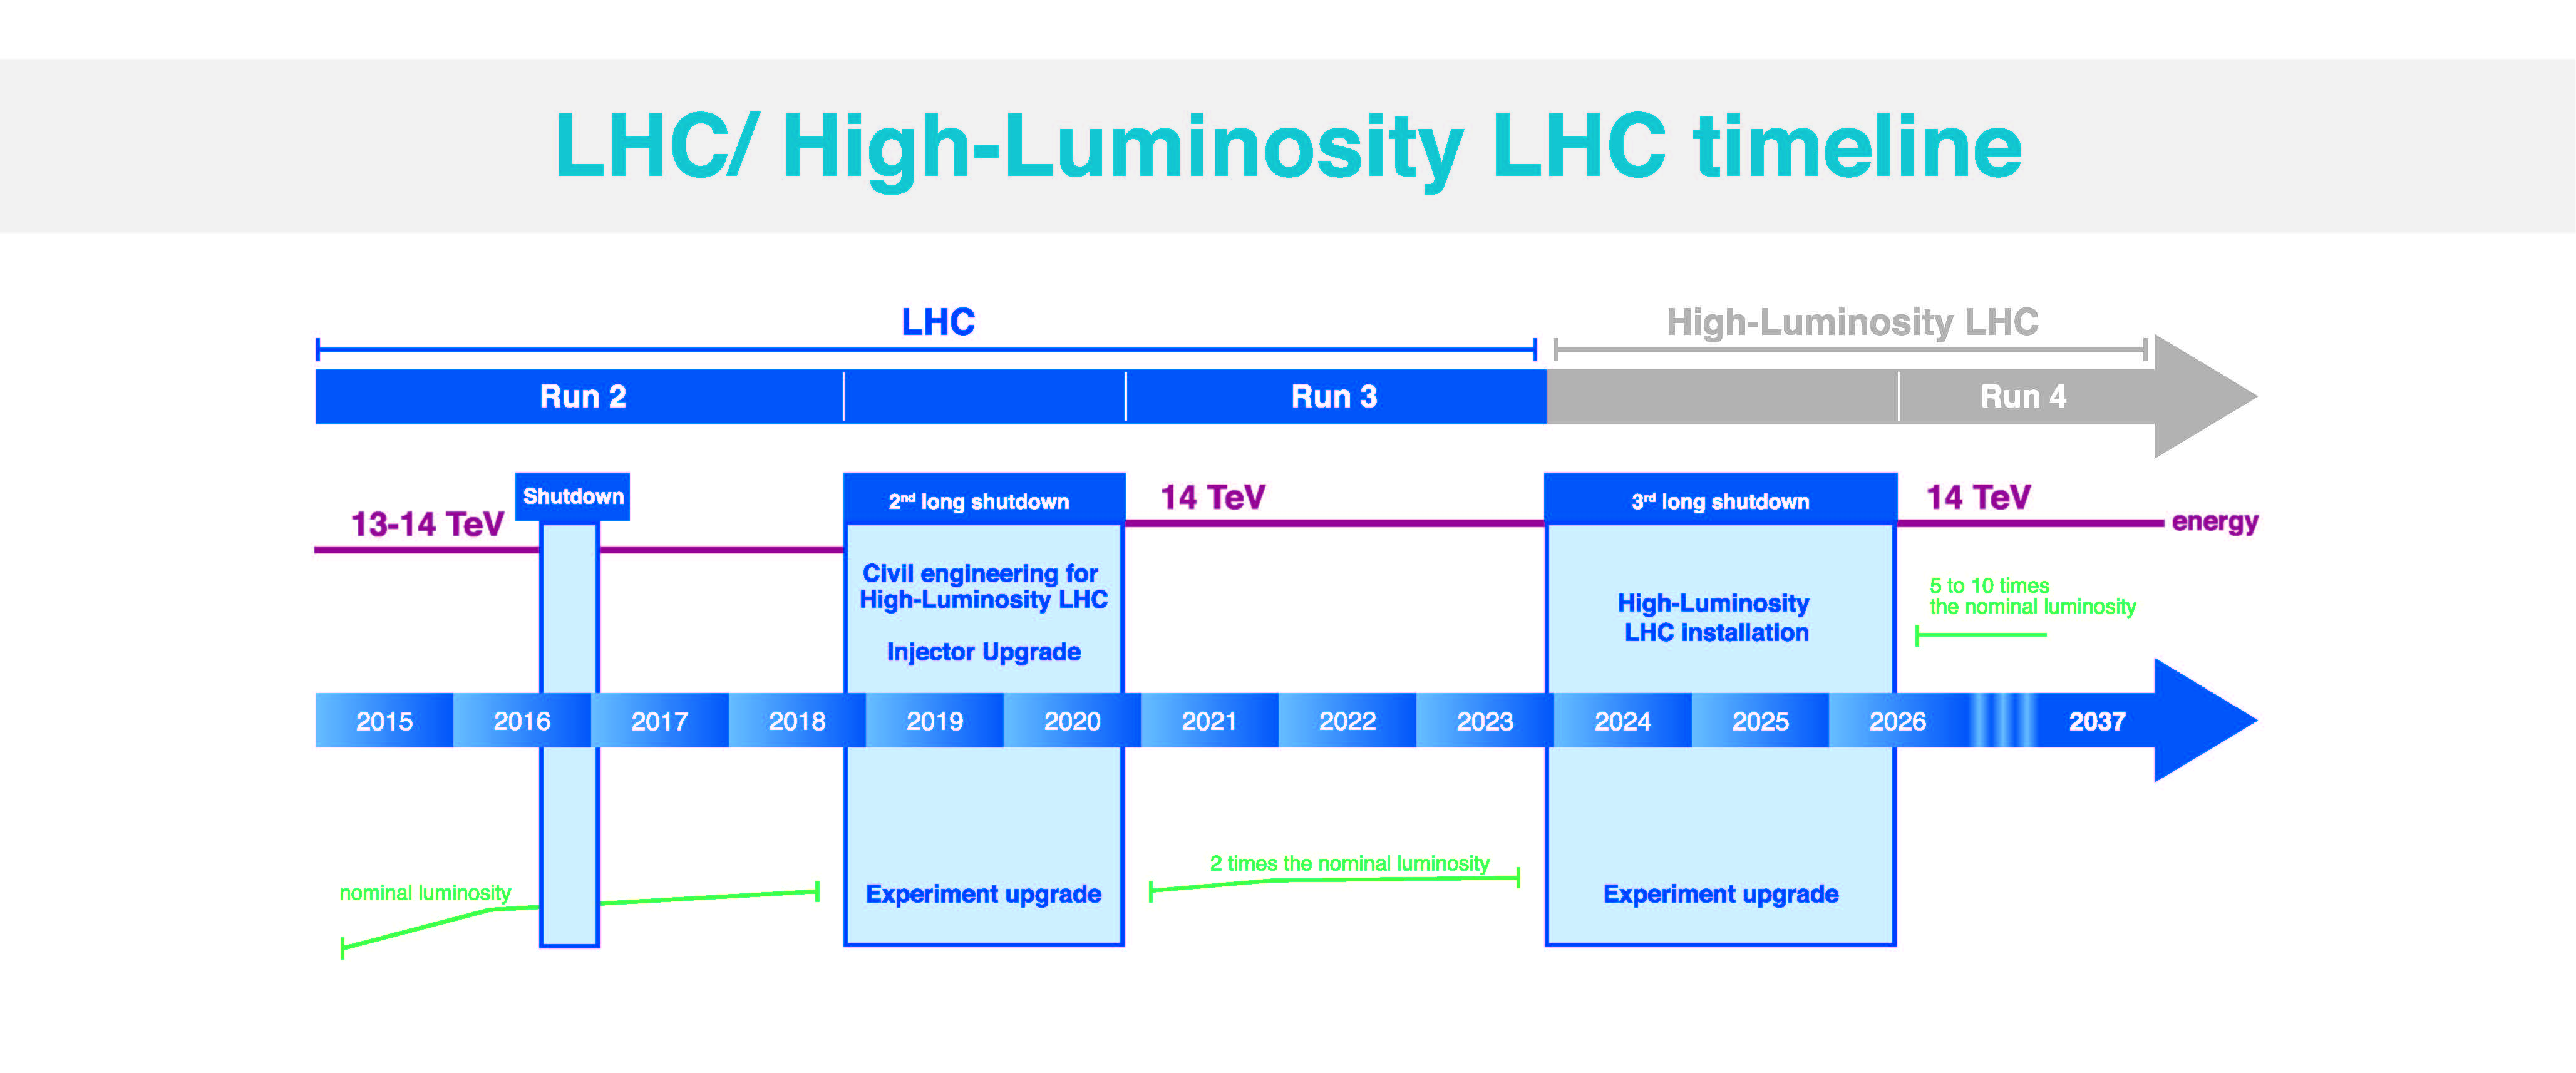
\includegraphics
              [scale=0.17,trim={6cm 1cm 6cm 6cm },clip=true]
              {p1-figs/hl-plan.jpg}
            \end{figure}
          \end{column}
          \end{columns}
        
        \end{minipage}  

    }

    \frame{
      \frametitle{High Luminosity LHC \& ITk Upgrades}
      %

        \begin{columns}[T,onlytextwidth]
        \begin{column}{.54\textwidth}

        \begin{block}{ $x10$ increase in instantaneous luminosity! }
            \begin{itemize}
              \item $L = $\num{1e73} fb$^{-1}$ s$^{-1} \rightarrow 
                     L = $ \num{1e74} fb$^{-1}$ s$^{-1} $ \\
              \item \bf{More particles, more problems}
            \end{itemize}
          \end{block}

        \end{column}
        \begin{column}{.4\textwidth}
				  \vspace{-1.2cm}
					\begin{figure}
						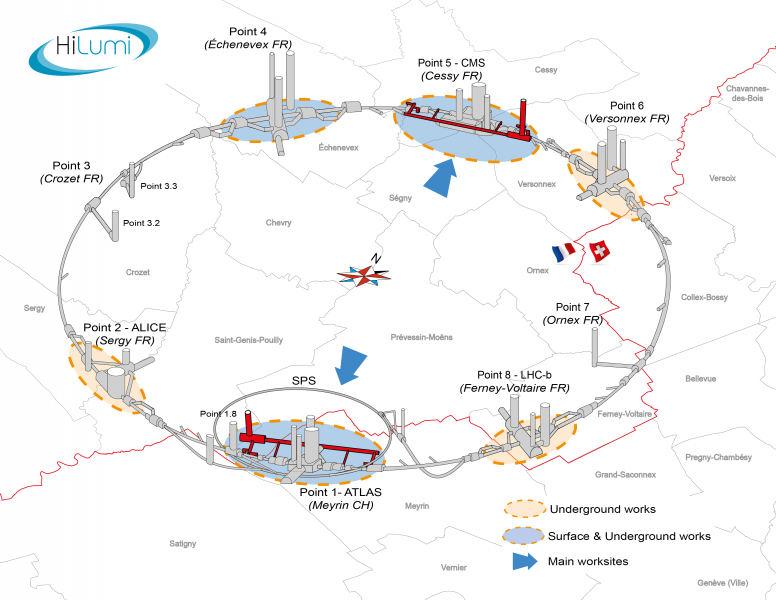
\includegraphics
						[width=\textwidth, height=.4\textheight]
						{p1-figs/hl-upgrade.png}
				 	\end{figure}

        \end{column}
        \end{columns}

        
        \begin{minipage}{\textwidth}
          \begin{columns}[T,onlytextwidth]
          \begin{column}{.5\textwidth}
            \begin{figure}
              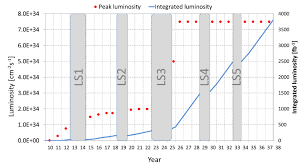
\includegraphics
              [height=.47\textheight]
              {p1-figs/hl.png}
            \end{figure}
          \end{column}
          \begin{column}{.6\textwidth}
            \vspace{0.5cm}
            \begin{figure}
              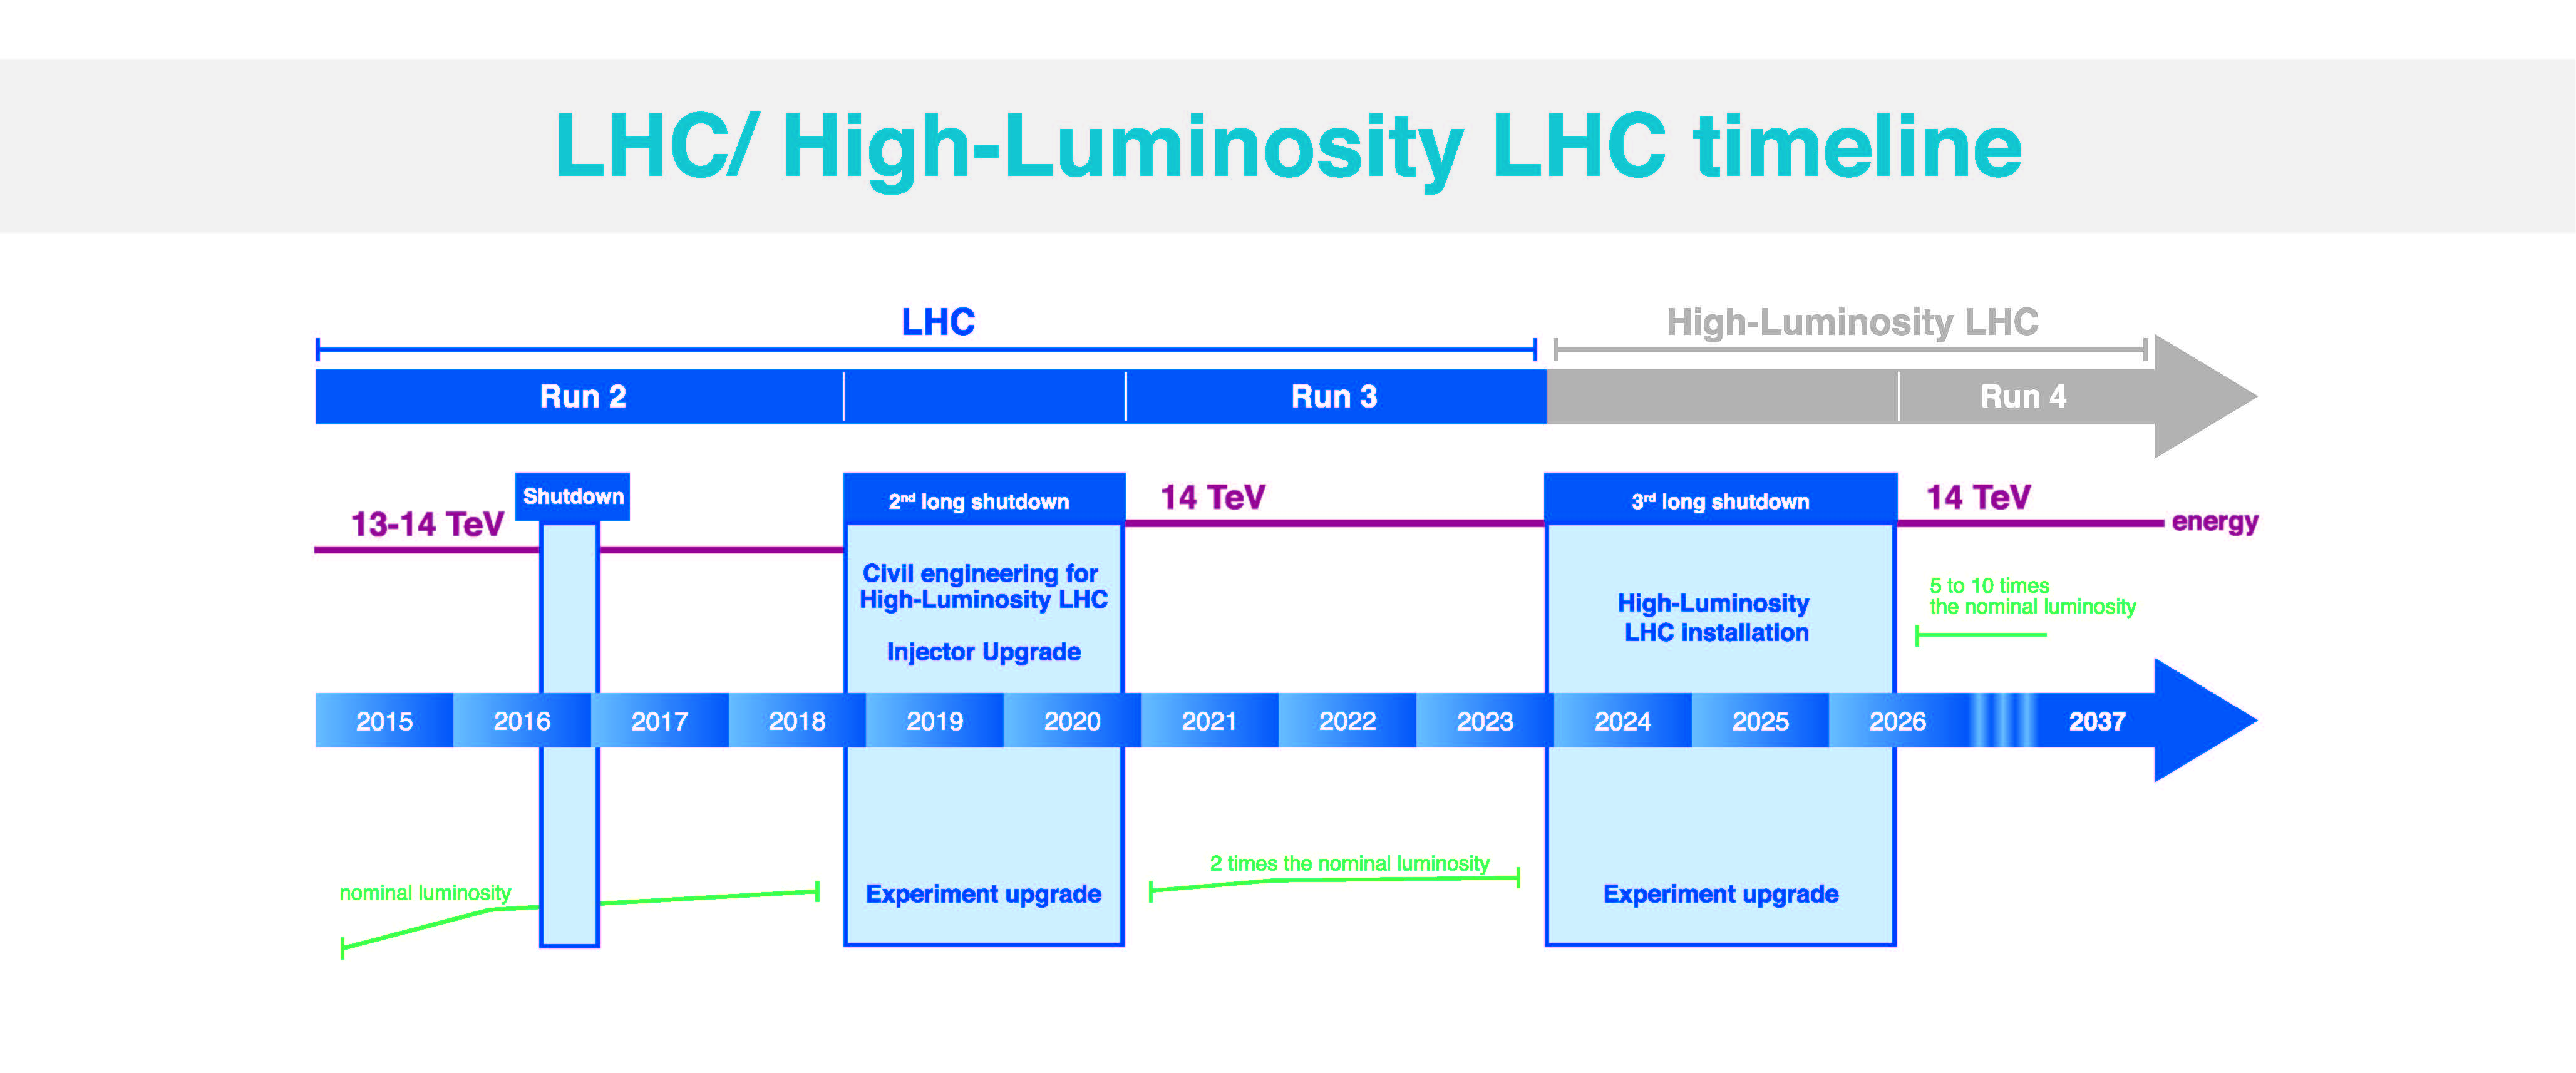
\includegraphics
              [scale=0.17,trim={6cm 1cm 6cm 6cm },clip=true]
              {p1-figs/hl-plan.jpg}
            \end{figure}
          \end{column}
          \end{columns}
        
        \end{minipage}  

    }
    
    \frame{
      \frametitle{High Luminosity LHC \& ITk Upgrades}
      %

        \begin{columns}[T,onlytextwidth]
        \begin{column}{.54\textwidth}

        \begin{block}{ $x10$ increase in instantaneous luminosity! }
            \begin{itemize}
              \item $L = $\num{1e73} fb$^{-1}$ s$^{-1} \rightarrow 
                     L = $ \num{1e74} fb$^{-1}$ s$^{-1} $ \\
              \item \bf{More particles, more problems}
            \end{itemize}
          \end{block}

        \end{column}
        \begin{column}{.4\textwidth}
				\vspace{-1.2cm}
					\begin{figure}
						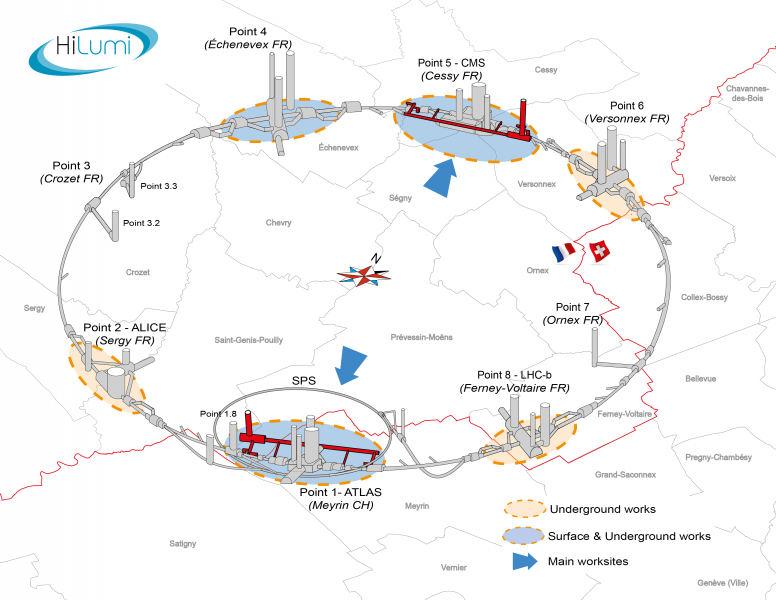
\includegraphics
						[width=\textwidth, height=.4\textheight]
						{p1-figs/hl-upgrade.png}
				 	\end{figure}

        \end{column}
        \end{columns}

        \begin{minipage}{\textwidth}
          \begin{block}{ The inner detector has insufficient:}
            \begin{itemize}
                \item radiation hardness
                \item granularity
                \item readout bandwidth
                \item trigger readout speed/storage
            \end{itemize}
          \end{block}
        \end{minipage}  

    }
    
    \frame{
      \frametitle{High Luminosity LHC \& ITk Upgrades}
      %

        \begin{columns}[T,onlytextwidth]
        \begin{column}{.54\textwidth}

        \begin{block}{ $x10$ increase in instantaneous luminosity! }
            \begin{itemize}
              \item $L = $\num{1e73} fb$^{-1}$ s$^{-1} \rightarrow 
                     L = $ \num{1e74} fb$^{-1}$ s$^{-1} $ \\
              \item \bf{More particles, more problems}
            \end{itemize}
          \end{block}

        \end{column}
        \begin{column}{.4\textwidth}
				\vspace{-1.2cm}
					\begin{figure}
						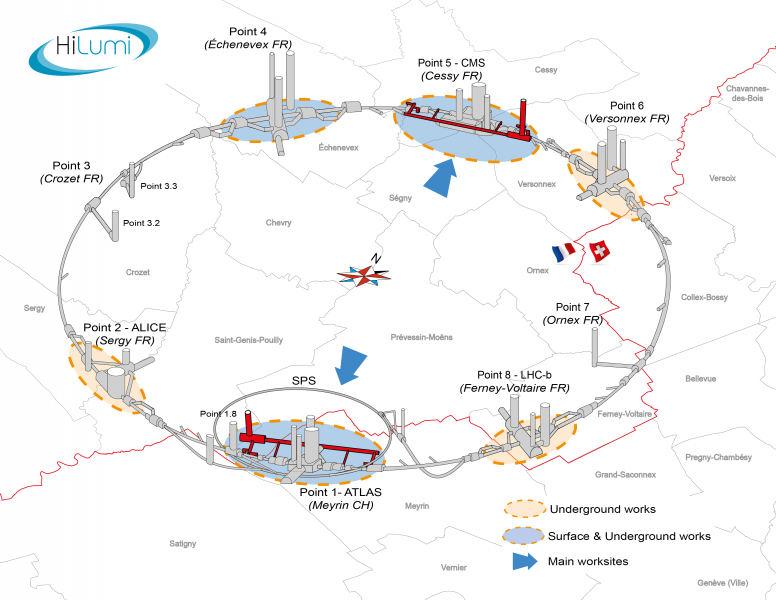
\includegraphics
						[width=\textwidth, height=.4\textheight]
						{p1-figs/hl-upgrade.png}
				 	\end{figure}

        \end{column}
        \end{columns}

        \begin{minipage}{\textwidth}
          \begin{block}{ The inner detector has insufficient:}
            \begin{itemize}
              \item radiation hardness: HL-LHC will deliver 4000 fb$^{-1}$  fluence. 
                    ID PIX is designed for 400 fb$^{-1}$, ID SCT for 700 fb$^{-1}$, 
                    IBL for 800 fb$^{-1}$
            \end{itemize}
          \end{block}
        \end{minipage}  

    }
    
    \frame{
      \frametitle{High Luminosity LHC \& ITk Upgrades}
      %

        \begin{columns}[T,onlytextwidth]
        \begin{column}{.54\textwidth}

        \begin{block}{ $x10$ increase in instantaneous luminosity! }
            \begin{itemize}
              \item $L = $\num{1e73} fb$^{-1}$ s$^{-1} \rightarrow 
                     L = $ \num{1e74} fb$^{-1}$ s$^{-1} $ \\
              \item \bf{More particles, more problems}
            \end{itemize}
          \end{block}

        \end{column}
        \begin{column}{.4\textwidth}
				\vspace{-1.2cm}
					\begin{figure}
						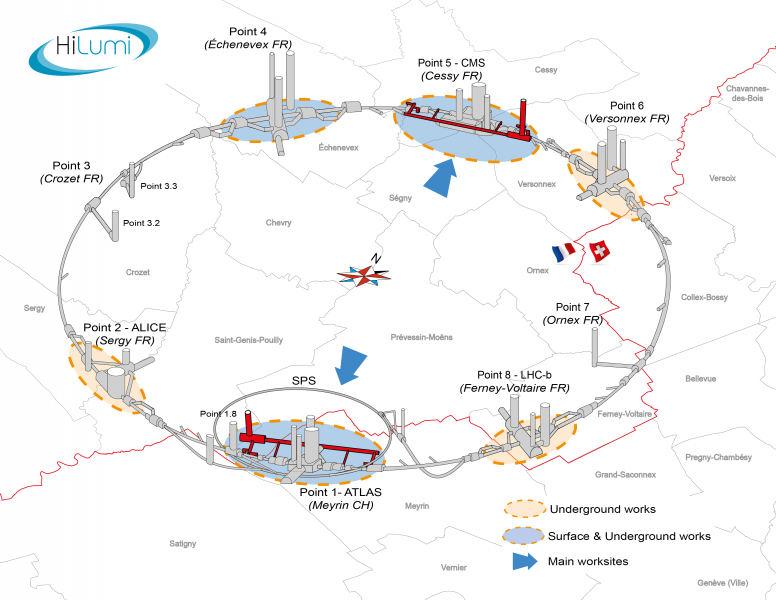
\includegraphics
						[width=\textwidth, height=.4\textheight]
						{p1-figs/hl-upgrade.png}
				 	\end{figure}

        \end{column}
        \end{columns}

        \begin{minipage}{\textwidth}
          \begin{block}{ The inner detector has insufficient:}
            \begin{itemize}
              \item granularity: Increasing fluence means higher granularity is needed to maintain performance; compensate for instrinsic dead time
            \end{itemize}
          \end{block}
        \end{minipage}  

    }
    
    \frame{
      \frametitle{High Luminosity LHC \& ITk Upgrades}
      %

        \begin{columns}[T,onlytextwidth]
        \begin{column}{.54\textwidth}

        \begin{block}{ $x10$ increase in instantaneous luminosity! }
            \begin{itemize}
              \item $L = $\num{1e73} fb$^{-1}$ s$^{-1} \rightarrow 
                     L = $ \num{1e74} fb$^{-1}$ s$^{-1} $ \\
              \item \bf{More particles, more problems}
            \end{itemize}
          \end{block}

        \end{column}
        \begin{column}{.4\textwidth}
				\vspace{-1.2cm}
					\begin{figure}
						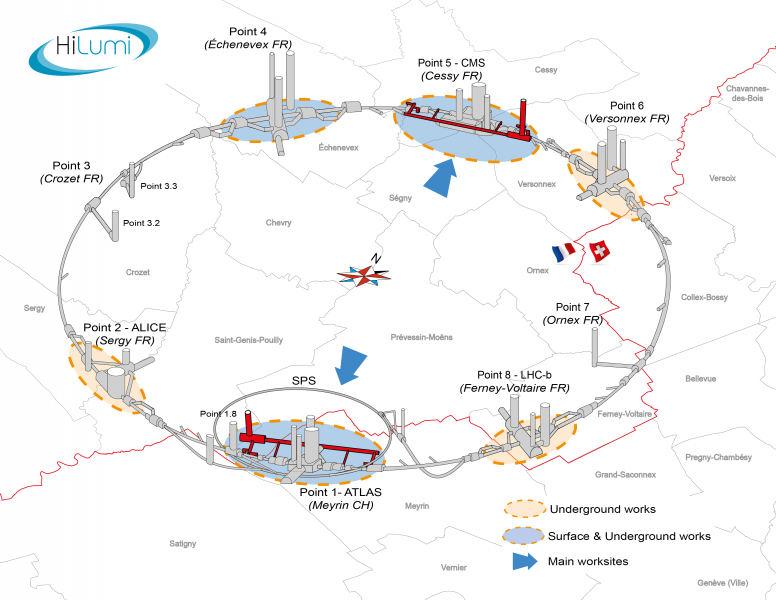
\includegraphics
						[width=\textwidth, height=.4\textheight]
						{p1-figs/hl-upgrade.png}
				 	\end{figure}

        \end{column}
        \end{columns}

        \begin{minipage}{\textwidth}
          \begin{block}{ The inner detector has insufficient:}
            \begin{itemize}
                \item readout bandwidth: HL-LHC will roughly quadruple ID designed bandwidth saturation
            \end{itemize}
          \end{block}
        \end{minipage}  

    }
    
    \frame{
      \frametitle{High Luminosity LHC \& ITk Upgrades}
      %

        \begin{columns}[T,onlytextwidth]
        \begin{column}{.54\textwidth}

        \begin{block}{ $x10$ increase in instantaneous luminosity! }
            \begin{itemize}
              \item $L = $\num{1e73} fb$^{-1}$ s$^{-1} \rightarrow 
                     L = $ \num{1e74} fb$^{-1}$ s$^{-1} $ \\
              \item \bf{More particles, more problems}
            \end{itemize}
          \end{block}

        \end{column}
        \begin{column}{.4\textwidth}
				\vspace{-1.2cm}
					\begin{figure}
						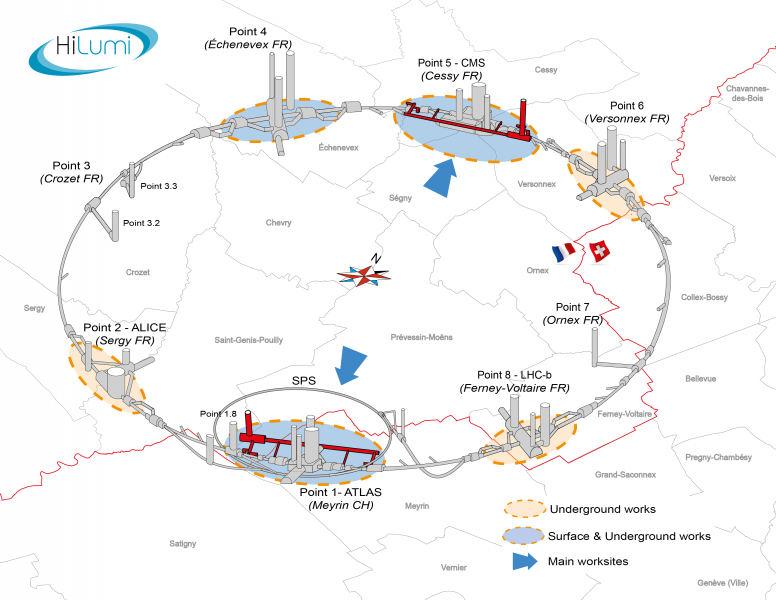
\includegraphics
						[width=\textwidth, height=.4\textheight]
						{p1-figs/hl-upgrade.png}
				 	\end{figure}

        \end{column}
        \end{columns}

        \begin{minipage}{\textwidth}
          \begin{block}{ The inner detector has insufficient:}
            \begin{itemize}
              \item trigger readout speed/storage: readout chain must accomadate much higher hardware (level 1) trigger rate
            \end{itemize}
          \end{block}
        \end{minipage}  

    }
    
    \frame{
      \frametitle{High Luminosity LHC \& ITk Upgrades}
      %

        \begin{columns}[T,onlytextwidth]
        \begin{column}{.54\textwidth}

        \begin{block}{ $x10$ increase in instantaneous luminosity! }
            \begin{itemize}
              \item $L = $\num{1e73} fb$^{-1}$ s$^{-1} \rightarrow 
                     L = $ \num{1e74} fb$^{-1}$ s$^{-1} $ \\
              \item \bf{More particles, more problems}
            \end{itemize}
          \end{block}

        \end{column}
        \begin{column}{.4\textwidth}
				\vspace{-1.2cm}
					\begin{figure}
						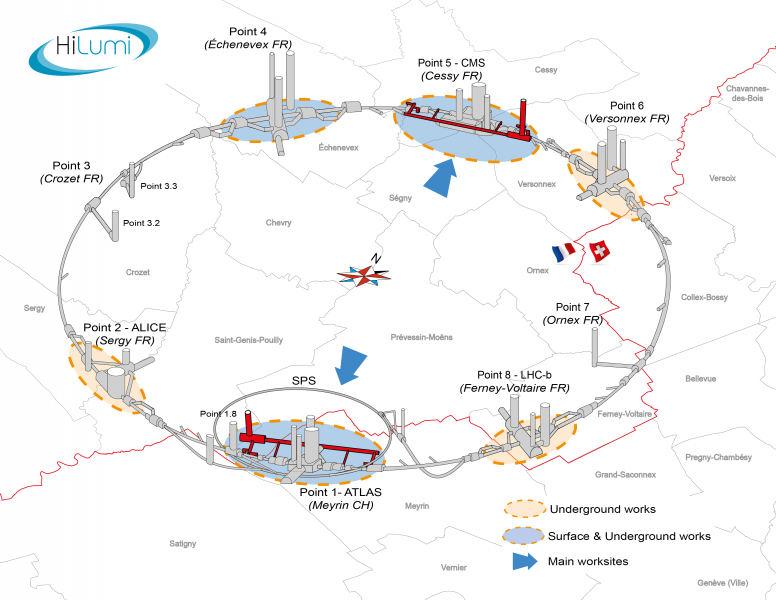
\includegraphics
						[width=\textwidth, height=.4\textheight]
						{p1-figs/hl-upgrade.png}
				 	\end{figure}

        \end{column}
        \end{columns}

        \begin{minipage}{\textwidth}
          \begin{block}{\large{\bf{Goal of ITk:}} }
            \large{\bf{Same or better performance than ID in 
            harsh environment of HL-LHC}} 
          \end{block}
        \end{minipage}  
    }

    \frame{ \frametitle{ITk design}
    
    \begin{minipage}{\textwidth}
    \begin{block}{ITk will have:}
    \begin{itemize}
      \item Strip detector: 70M channels (6M currently)
      \item Pixel detector: 600M channels (80M currently)
    \end{itemize}
    \end{block}
    \end{minipage}
    
    \begin{minipage}{\textwidth}
      \begin{columns}[T,onlytextwidth]
      \begin{column}{.4\textwidth}

        % design
				\begin{figure}
					\includegraphics
          [trim={0cm 0cm 0cm 0cm},clip,width=0.8\textwidth ]
					{example-image}
          \caption{Design of ITk}
			 	\end{figure}

      \end{column}
      \begin{column}{.4\textwidth}
				
        % rad length vs eta
        \begin{figure}
					\includegraphics
          [trim={0cm 0cm 0cm 0cm},clip,width=0.8\textwidth ]
					{example-image}
          \caption{ITk radiation length v. $\eta$}
			 	\end{figure}


      \end{column}
      \end{columns}
    \end{minipage}
    }


    \frame{
      \frametitle{ITk Design: Strip Detector}
      % ignoring pixel detector
        \begin{columns}[T,onlytextwidth]
        \begin{column}{.45\textwidth}

          \vspace{-0.5cm}
					\begin{figure}
						\includegraphics
            [trim={0cm 0cm 0cm 0cm},clip,width=1.2\textwidth ]
						{example-image}
				 	\end{figure}

        \end{column}
        \begin{column}{.4\textwidth}

          \begin{itemize}
              \item barrel staves
              \item endcap petals
          \end{itemize}

        \end{column}
        \end{columns}
    }
    
    \frame{
      \frametitle{Strip Detector Readout}
    }


   
    % ============================================================== %
    %
    % Our Progress
    %
    % ============================================================== %
    
    \section{Our Progress}
    \subsection{s1}
    \subsection{s2}
    
    \frame{
        \frametitle{ATLYS Board}
        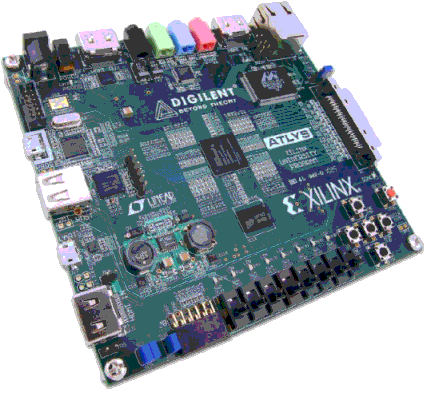
\includegraphics[width=0.5\paperwidth]{images/atlys_pic.png}
    }
    
    \frame{
        \frametitle{Obstacles}
        fuck
    }

    % ============================================================== %
    %
    % Acknowledgements
    %
    % ============================================================== %
    
    \section{Acknowledgements}
    

    \frame{
        \frametitle{Acknowledgements}

        \vspace{-2.0cm}


        We would like to acknowledge the University of Michigan Department of Physics,\\ specifically Jean Krisch, Tom Schwarz, and Steven Goldfarb. 

        We would also like to acknowledge the support of the Lounsbery foundation.   \\


        \begin{minipage}{\textwidth}

          \begin{tikzpicture}[remember picture, overlay]
            \node[anchor=south west, %anchor is bottom left corner of the graphic
                  xshift=2.4cm ]
           at (current page.south west) %left bottom corner of the page
            { 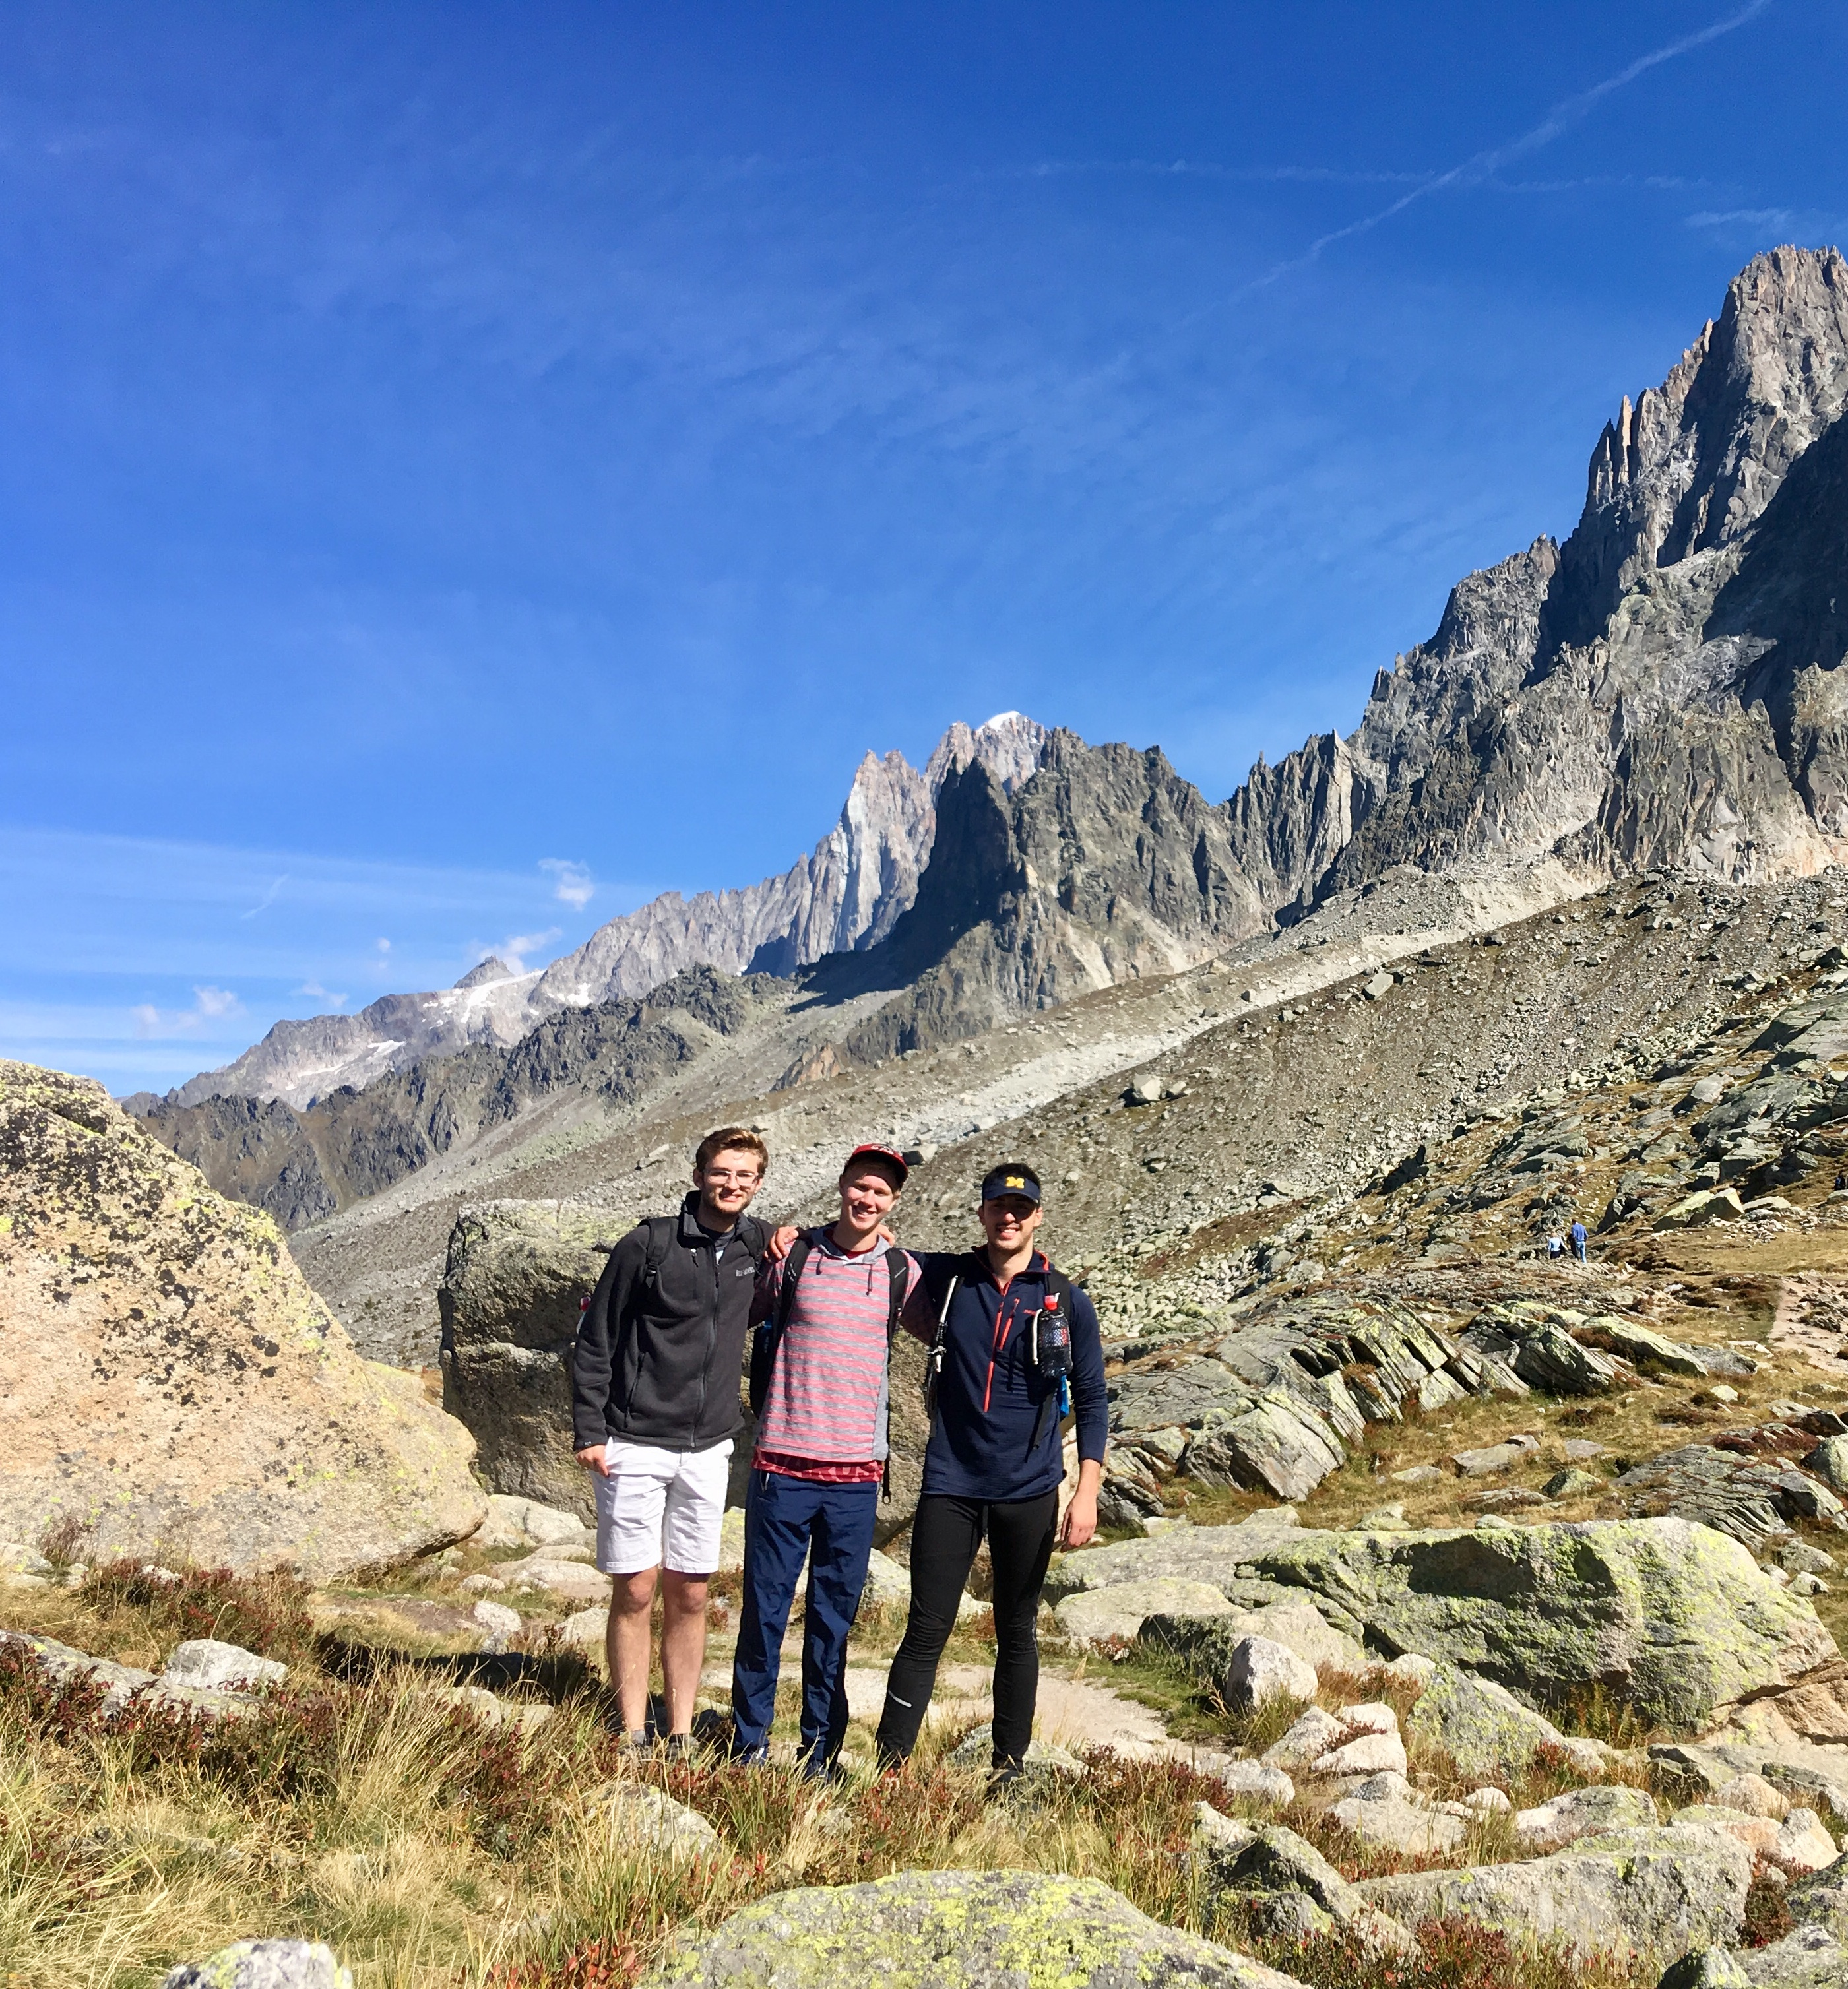
\includegraphics[scale=0.05,trim={0 0 0 35cm },clip]
            {p1-figs/cham.jpg} };

            \node[anchor=south east, %anchor is bottom left corner of the graphic
                  xshift=-2.4cm]
           at (current page.south east) %left bottom corner of the page
            {	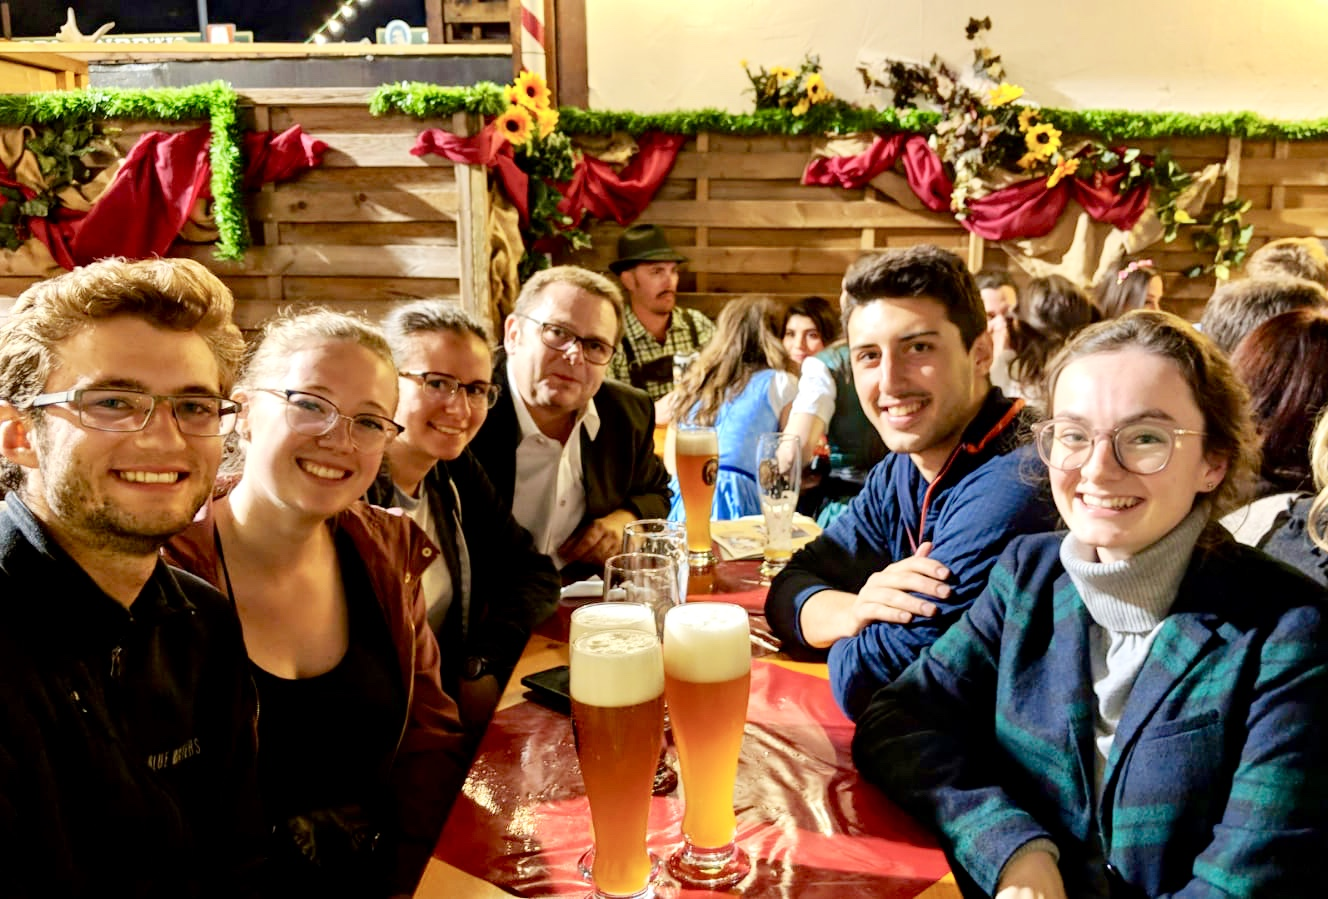
\includegraphics[width=0.33\paperwidth]{p1-figs/okto.jpg} };
          \end{tikzpicture}

        \end{minipage}  

    }

    \section{}
    \cernSplashWhite

\end{document}
